	Dans le cadre de notre étude du SPA, nous nous sommes consacrés à la structure du paquet SPA à envoyer afin qu'il répondent aux exigences du procédé. 
Nous souhaitons, en effet, que notre serveur SPA puisse authentifier les demandes, vérifier leurs intégrités et ne sois pas sensible aux attaques de type \emph{rejeu} et \emph{DoS}. 
Le schéma suivant satisferait ces exigences :

\begin{figure}[h]

\centerline{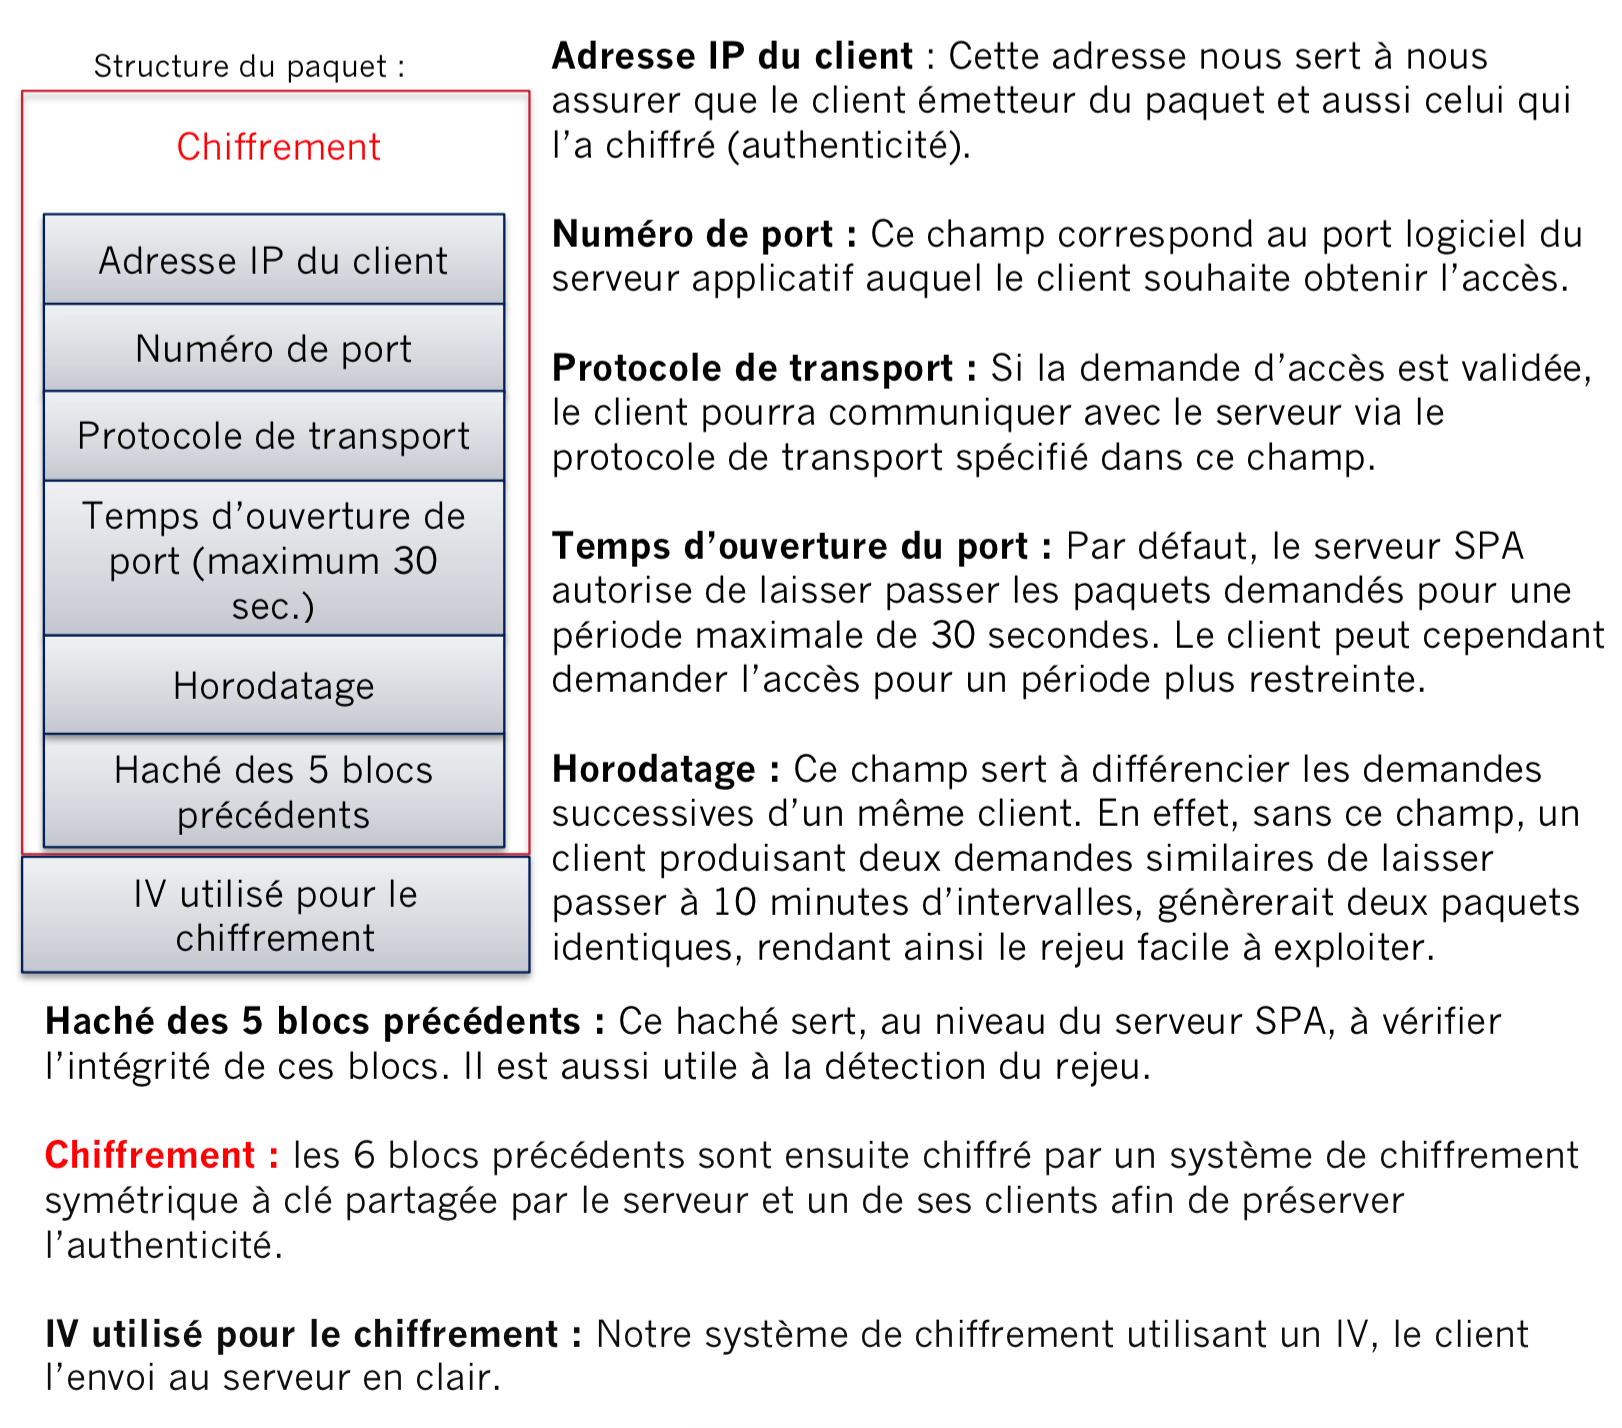
\includegraphics[scale=0.5]{paquet_spa}}
\caption{Schéma du champ de données d'un paquet SPA}

\end{figure}

\newpage


